
\subsection{Physics and properties of solids}
The most common distinction between solids is taking their resistivity as a criterion. We can distinguish three main categories for them - metals, semiconductors and isolators. Within that we can also provide temperature differences beneath them as for the metals, the resistivity goes down with the temperature increase and for the rest of them it is quite the opposite.

Also, as it will be later extended, when we light a semiconductor or an isolator we can clearly observe so called \textit{absorption threshold}. 
\begin{figure}[H]
\centering
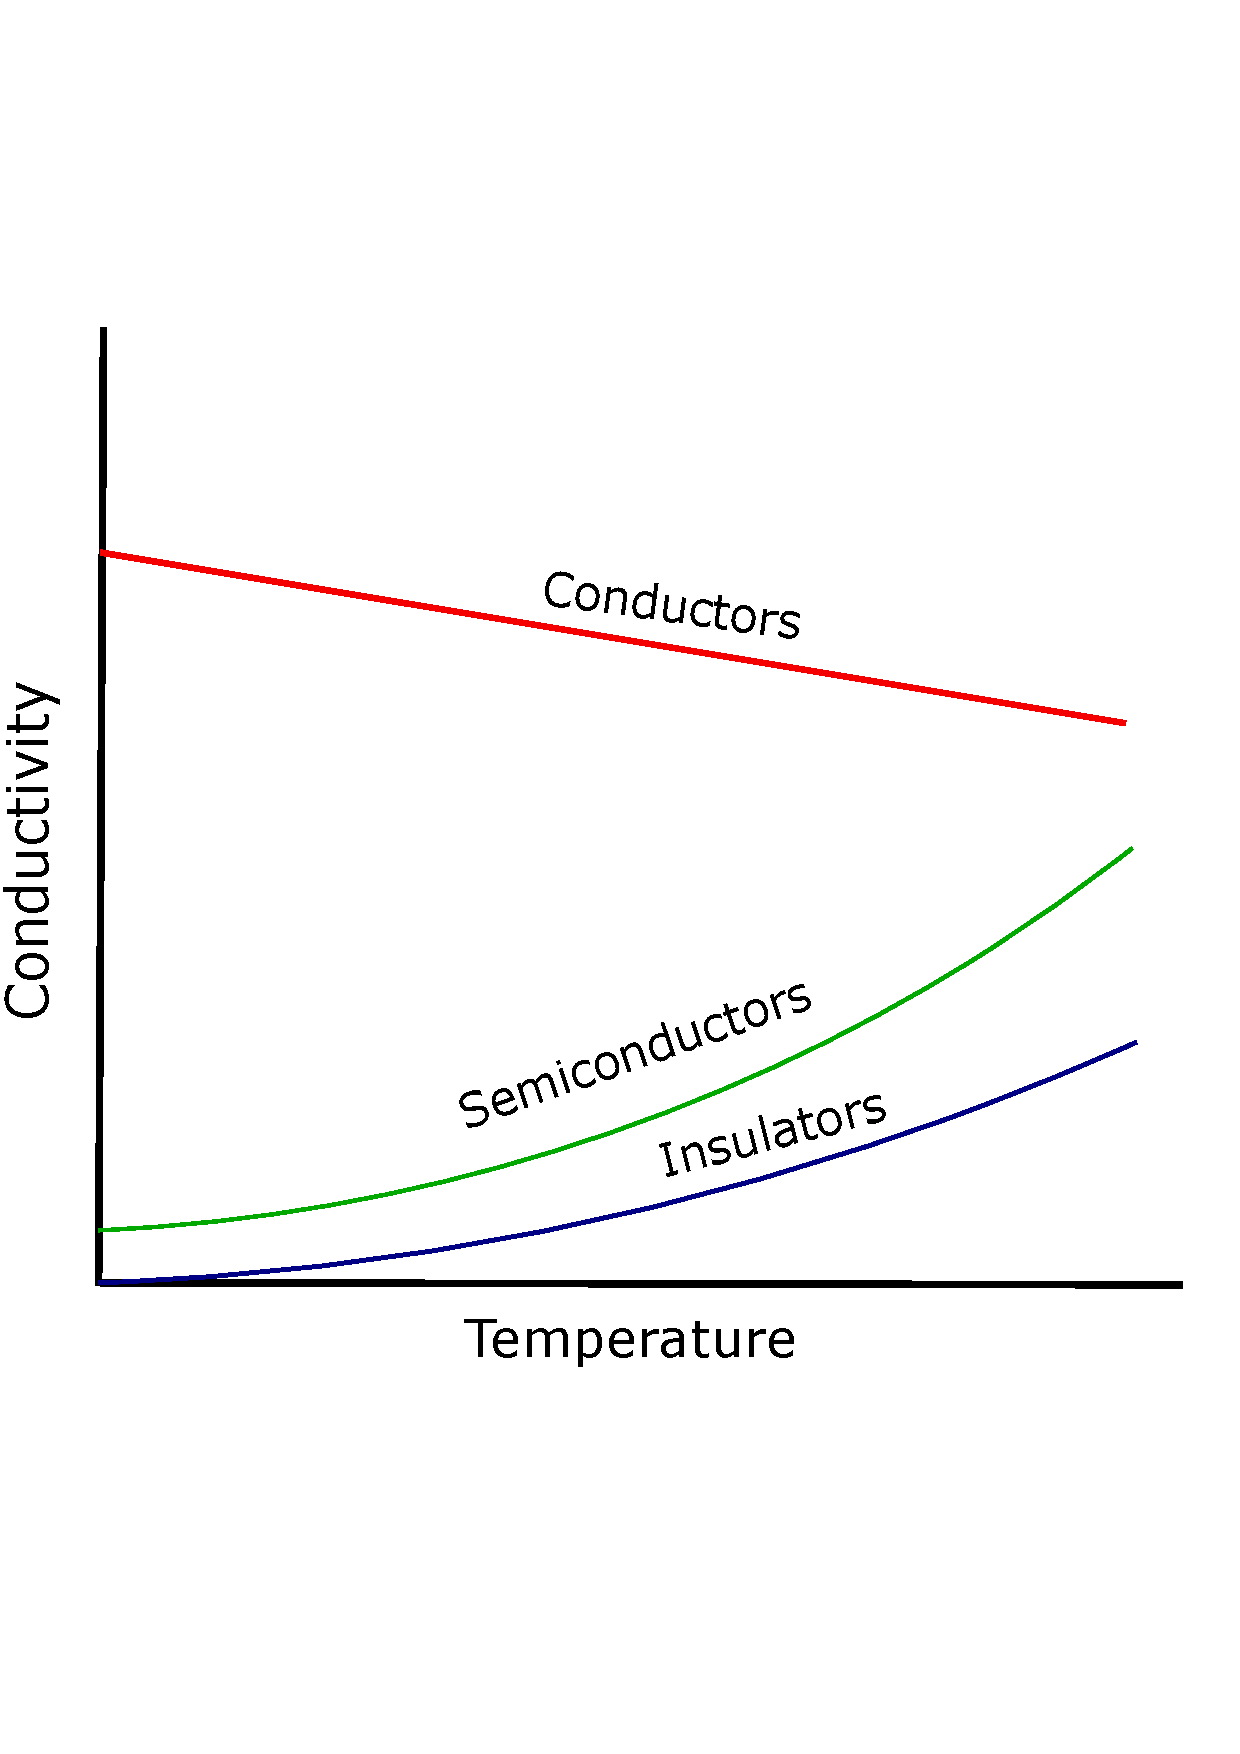
\includegraphics[scale=0.45]{Con_temp.pdf}
\caption{Demonstrations of conductivity behaviour of different types of solids}
\end{figure}
\subsection{Drude model of free carriers}
The discovery of electron in 1897 had the great impact on the first attempt to describe properties of solids. Fairly early, just three years later, Drude constructed his first theory which based on the usage of quite successful kinetic theory, which described the behaviour of gases. Starting with metals he imagined a gas of electrons which are identical solid spheres moving randomly in straight lines. They change directions by collisions and of course no other forces than that of the very quick collisions are taken into account. As metals are neutral, Drude deduced that much heavier and steady particles are compensating negative electron charge. Strictly, that kind of model provides us with the crystal structure but back then, Drude assumed (and for great deal of metals it's fairly true), that only valence electrons are important and they move freely through the whole metal. The basic assumptions for the model are:
\begin{enumerate}
\item Between collisions, interactions electron-electron and electron-ion are able to be neglected. The first one is called \textit{independent electron approximation} and the second is called \textit{free electron approximation}. 
\item Only the collisions are important. They are approximately instantaneous events that alter the velocity of the electron. The electron-electron scattering is one of the least important scattering mechanisms in metals. Nevertheless with others, very often, in describing conducting electrons it is not important to describe all mechanisms deeply. 
\item We can assume that the period in which an electron isn't making any collision is $\tau$ \textit{(relaxation time)} and thus the probability that electron is undergoing a collision in any infinitesimal time period dt is $\frac{dt}{\tau}$. This of course means that $\tau$ is average time and it is independent of both velocity and position $\rightarrow$ therefore also time. 
\item Thermal equilibrium is achieved only through collisions.
\end{enumerate}

\subsubsection{Electrical Conductivity}

Drude model can describe, with certain accuracy, the Ohm's law $V=IR$. Resistance R is a quantity which is dependent of the dimensions of the material, therefore resistivity, which has been mentioned before can be used.
\begin{equation}
\mathbf{E}=\rho\mathbf{j}
\end{equation}
The current density \textit{j} is the same as in former section, when we were describing Maxwells equations. If n electrons move with velocity \textbf{v} in time period dt and through area A we get that charge connected with that quantities is $-nevAdt$ so current density is:
\begin{equation}
\mathbf{j}=-ne\mathbf{v}
\label{eq:curr_dens_drud}
\end{equation}
and is just a net current because of random electron movement. 
Also, let's assume that electron has a velocity $\mathbf{v_0}$ at time $t_0$ just after a collision and additional velocity $\frac{-\mathbf{E}e\tau}{m}$ from the external field, we can take average through long time period. The random velocity $\mathbf{v_0}$ disappears and therefore, connecting with \ref{eq:curr_dens_drud} we get that:
\begin{equation}
\mathbf{j}=\sigma\mathbf{E}
\end{equation}
\begin{equation}
\sigma=\frac{ne^2\tau}{m}
\end{equation}
This tells us about the linear dependence of \textbf{j} on \textbf{E}. Note that $\tau = \frac{m}{\rhone^2}$ because $\tau = 1/\rho$.
Drude model was a first and simple model used in describing solid state materials. As simple as it is, it can yet provide some accurate results. 








\subsection{Crystal structure and Bloch theorem}

\subsection{Energy structure}

\subsection{Bigger world of carriers}

\subsection{Non-equilibrium processes}

\subsection{Carrier injection}

\subsection{Recombination}

\subsection{Semiconductor junctions}

